\subsection{Fast Eagle}
    \subsubsection{Definición}
      \paragraph{El módulo Fast Eagle formará parte de la arquitectura final de Ambienta2MX. El propósito principal de este módulo es brindar la información cartográfica de México por medio de un servicio expuesto, considerando latitud, longitud o nombre de la localidad deseada.}
      \paragraph{Fast Eagle se encargará de la lectura, carga, verificación y resolución de los archivos brindados por el (Instituto Nacional de Estadística y Geografía) INEGI en la información pública que tiene de la cartografía del territorio nacional.}
      \paragraph{El proceso de toma de datos del INEGI será ejecutado sólo una vez al inicio o primer despliegue del sistema. Esto debido a que la cartografía no deberá ser procesada de forma dinámica. Se usará un modelo de datos persistido Mongo para sus posteriores consultas.}
      \paragraph{La información que proporciona el INEGI carece de campos esenciales para la estandarización de los información cartográfica, para dar solución a ese contratiempo se hará uso de servicios externos que ya cuentan con información definida, es decir, que su información ha pasado bajo un cierto proceso de limpieza y regulación, por ejemplo, los servicios de Google Places API.}
      \paragraph{En caso de que no exista la información deseada por el usuario o algún otro módulo del sistema en la cartografía (base de datos llamada Places), Fast Eagle tratará de resolver la información en fuentes externas, persistiendo el modelo resuelto y regresando esa información al solicitante.}
    \subsubsection{Diagrama de sequencias}
    \begin{center}
      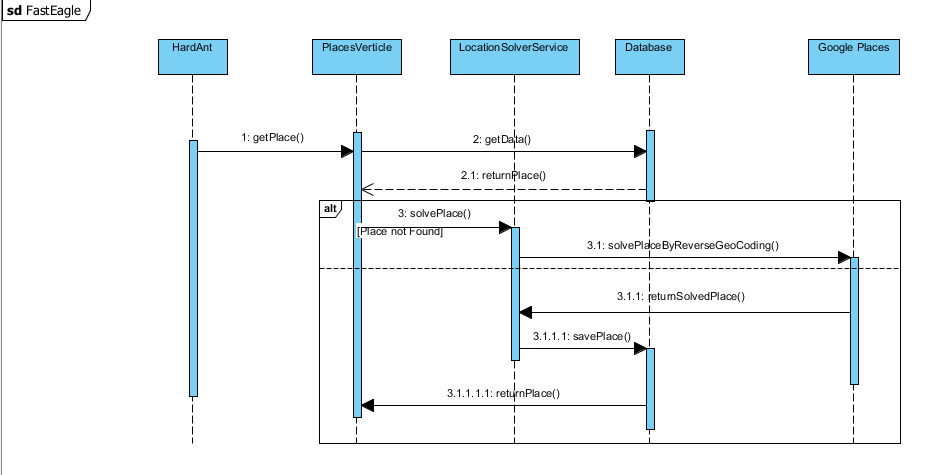
\includegraphics[width=16cm,height=10cm]{./images/FastEagleSequenceDiagram}
    \end{center}
    \subsubsection{Diagrama por bloques}
      \paragraph{Fast Eagle contará con varios procesos a ser desarrollados, la integración de cada proceso y su respectiva integración dará solución a un problema de estandarización, resolución y consulta de datos geográficos vía Latitud, Longitud y Ubicación.}
    \newpage
      \begin{landscape}
        \begin{figure}[b!]
        \centering
        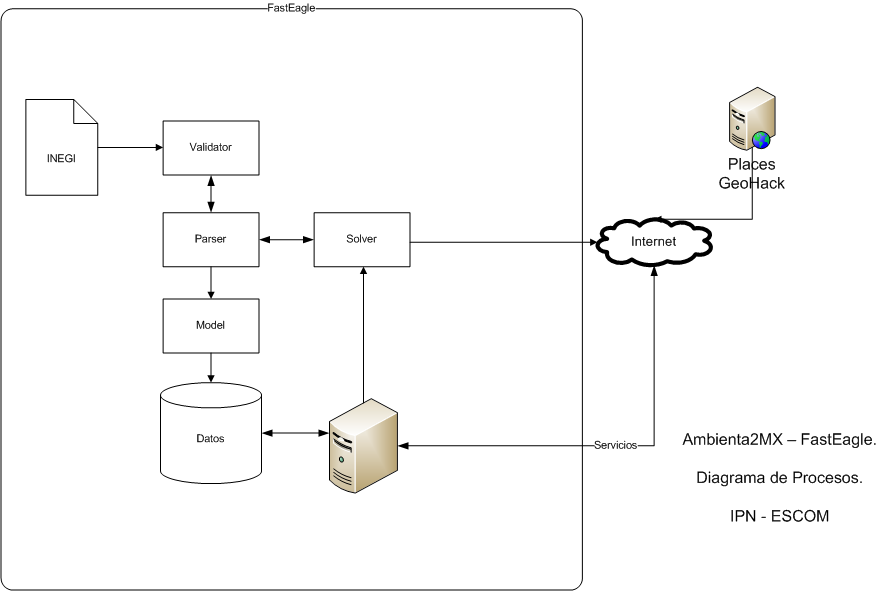
\includegraphics[width=22.5cm,height=12cm]{./images/DiagramaFastEagle.png}
        \caption{Diagrama por bloques de Fast Eagle}
      \end{figure}
      \end{landscape}
    \newpage
    \paragraph{En el diagrama se muestran cuatro módulos básicos, estos forman parte del núcleo de Fast Eagle, también podemos observar que se cuenta con la interacción de servicios de terceros como Google Places,  también se cuenta con la exposición de los servicios a través de un servidor  web.}
    \paragraph{El módulo de Validación \textbf{\emph{Validator}}, será el encargado de tomar las fuentes que el INEGI brinda al público en general en forma de archivos CSV, y realizar un proceso de validación a los datos que éstos tienen.}
    \paragraph{El módulo indicará que datos necesitan una resolución y cuáles pueden ser estandarizados y posteriormente almacenados en la base de datos.}
    \paragraph{\textbf{\emph{Parser}} tomará los datos que el proceso de validación le arroje para transformar al estado propuesto por el equipo de trabajo (Véase modelo de datos). Considerando un proceso de resolución en caso de que la información proporcionada por el INEGI se encuentre incompleta no sea válida.}
    \paragraph{Para toda la información que carezca de datos correctos \textbf{\emph{Solver}} buscará una resolución en servicios de terceros, después de la resolución, los datos serán guardados en el gestor de bases de datos bajo el formato propuesto por el equipo de trabajo.}
    \paragraph{\textbf{\emph{Model}} es la capa de interacción con la base de datos, ésta se encarga de las operaciones mejor conocidas como CRUD (Create, Read, Update and Delete),  persistiendo la información en MongoDB.}
    \paragraph{Para poder exponer los datos, se hará uso de un servidor web minimalista orientado a micro servicios, éste será un servicio público que formará parte de la infraestructura final de Ambienta2MX.}
    \paragraph{El servicio expuesto se encargará de las búsquedas a nivel base de datos y en caso de no encontrar la información buscará en terceros para poder agregarla a la base de datos y así ir mejorando el contenido de nuestro índice cartográfico.}